\newcommand{\Projekt}{LEGO GCT Pflichtenheft}

\documentclass[a4paper,12pt]{article}
\usepackage[a4paper,left=1cm,right=1cm,top=2cm,bottom=2cm]{geometry}

\usepackage[utf8]{inputenc}
\usepackage[ngerman]{babel}
\usepackage[T1]{fontenc}
\usepackage{booktabs}
\usepackage{multirow}
\usepackage{graphicx}
\usepackage{tabularx}
\usepackage{longtable}

\title{\Projekt}
\author{Caner Kara, Dennis Behrendt, Sven Wolf, Tim Sibum, Hannes Scherer,Tim Turowski}
\date{\today}

\begin{document}

\maketitle


\includegraphics[width=18cm]{pictures/LogoRiesig.png}

\newpage
\section{Änderungshistorie}

\begin{flushleft}
		\begin{longtable}{p{2cm}p{2cm}p{3cm}p{9cm}c}
        %% Tabellenkopf
            \toprule
            \textbf{Version} & \textbf{Datum} & \textbf{Autor} & \textbf{Änderungen}\\
            \midrule\endfirsthead
            \toprule
            \textbf{Version} & \textbf{Datum} & \textbf{Autor} & \textbf{Änderungen}\\
            \midrule\endhead
        %% Tabelleninhalte
            	Version 1.0 & 23.04.2023 & Tim Turowski & Git-Repository angelegt und Pflichtenheft Tex-Dokument \\ \midrule
				Version 1.1 & 26.04.2023 & Tim Silbum & ERM und UML Diagramm zur Datenstruktur eingefügt \\ \midrule
				Version 1.2 & 26.04.2023 & Hannes Scherer & Frontend Prototypen entwickelt \\ \midrule
				Version 1.3 & 27.04.2023 & Tim Silbum & Sequenzdiagramm, Zustandsdiagramm und GUI Skizze \\ \midrule
 				Version 1.4 & 28.04.2022 & Tim Turowski & Bilder ins Pflichtenheft eingefügt und Tabellen angepasst \\ \midrule
				Version 1.5 & 02.05.2023 & Dennis Behrendt & Bezogen auf das erste Feedback: Inhalte korrigiert und Ausformulierungen angepasst \\ \midrule
				Version 1.6 & 03.05.2023 & Hannes Scherer & Bezogen auf das erste Feedback: Frontend Prototypen angepasst \\ \midrule
				Version 1.7 & 06.05.2023 & Tim Turowski & Nach Problemen beim mergen im Repository: Pflichtenheft ist eigenständiges Dokument \\ \midrule
				Version 1.8 & 07.05.2023 & Tim Turowski & Inhalte der Projektmitglieder eingefügt für morgiges Meeting \\ 
            \bottomrule
    \end{longtable}

\end{flushleft}

\newpage

\tableofcontents

\newpage

\section{Zielbestimmung}

Heutzutage günstig Lego-Sets zu erwerben kann auf mehreren Ebenen ein wohlüberlegtes Unterfangen sein. Welche der Lego-Händler bieten die Sets günstig an? Ist es günstiger sich die Einzelteile des Sets einzeln zu bestellen? Was ist wenn bestimmte Einzelteile nicht mehr verfügbar sind? \newline
Das Ziel des Projekts ist genau diese Fragestellungen, durch die Entwicklung eines Tools zur Ermittlung der günstigsten Anbieter, zu beantworten. Das Tool soll dabei auch in der Lage sein, abzuwägen, ob es günstiger ist, das Set oder Einzelteile zu kaufen und zu kombinieren.

\subsection{Musskriterien}
\begin{enumerate}
\item Es soll eine Datenbank mit Stücklisten und Bauteilen geben
\item Die PDF-Bauanleitungen der Lego-Sets sollen mit OCR auslesbar sein
\item Ein Crawler bezieht die Preise der unterschiedlichen Händler zur Laufzeit der Suche
\item  Ein Preisvergleich unter den Händlern, im Bezug auf Kauf eines Sets oder der jeweiligen Einzelteile, findet statt
\item Darstellung des Tools als graphische Oberfläche. (Startseite, Benuterverwaltung, Preisvergleich, Warenkorb)
\item Es soll möglich sein Benutzeraccounts anzulegen und diese zu verwalten
\item Drei feste Händler sollen beim Vergleich berücksichtigt werden
\item Auf nicht verfügbare Einzelteile sollte hinreichend hingewiesen werden.
\item Die Lieferkosten sollen beim Preisvergleich berücksichtigt werden.
\item Bei der Ausgabe des Vergleichs soll eine Verlinkung zum Produkt, sowie eine Liste der Bauteile, angezeigt werden.
\end{enumerate}

\subsection{Kannkriterien}
\begin{enumerate}
\item Plattform sollte auch auf Mobilgeräten gut dargestellt sein
\item Mehr Händler sollten noch mit aufnehmbar sein
\end{enumerate}

\subsection{Wunschkriterien}
\begin{enumerate}
\item Einzelteile die besonders selten/teuer sind sollten gesondert aufgelistet werden
\item Filterfunktion um zum Beispiel Figuren rauszufiltern
\item Sticker berücksichtigen
\item Eigene Bauanleitung auslesen lassen
\item Aktuelle Angebote hervorheben
\item Dashboard: Statistiken zum Suchverhalten unserer Benutzer / Wie erfolgreich war unser Programm?
\item Es sollte eine Funktion geben um den Warenkorb beim entsprechenden Händler automatisch befüllen zu lassen
\end{enumerate}

\subsection{Abgrenzungskriterien}
\begin{enumerate}
\item Unser Produkt wird keine Verkaufsplattform haben
\item Keine Bevorzugung von Händlern
\item Wir berücksichtigen keine nicht offiziellen Klemmbausteine
\item Website ist nur für deutschsprachige Benutzer
\item Alte Sets ohne Stückliste in der Anleitung können nicht berücksichtigt werden (2006)
\item Wir berücksichtigen keine Retailpreise
\item Nur Bauanleitungen aus der Lego-Datenbank sollen aufgenommen werden
\end{enumerate}

\section{Produkteinsatz}
 Das Produkt soll Benutzer bei Kaufentscheidung unterstützen, außerdem unterstützt es die Benutzer Sets zu bauen die aus irgendwelchen Gründen nicht mehr verfügbar sind.\newline
Das Tool ist für Lego-Enthusiasten und Sammler gedacht, die nach dem günstigsten Angebot suchen. Das Tool kann auch von Einzelpersonen oder Unternehmen genutzt werden, die große Mengen an Lego-Sets kaufen möchten. \newline

\section{Produktfunktionen}

\subsection{Benutzersicht}

/F10/ \newline
Geschäftsprozess: Über eine Suchmaske können Lego Setnummern eingeben\newline
Vorbedingung: User befindet auf der Website des LegoGCT\newline
Nachbedingung: Nach der Eingabe wird die Datenbank auf die Existenz des Lego Sets geprüft\newline
Fehlerfall: Die Eingegebene Setnummer stimmt nicht mit einer in der Datenbank vorhanden Setnummer überein. Oder Syntaxfehler führt zur falschen Eingabe\newline
Anwender: Akteur im Kontext der Webapplikation\newline
Beschreibung: Über die Suchfunktion kann der Benutzer eine Setnummer eingeben.\newline\newline
/F20/\newline
Geschäftsprozess: Registrierung auf der Webplattform\newline
Vorbedingung: User befindet auf der Website des LegoGCT und hat den Registrieren Button gedrückt\newline
Nachbedingung: User konnte sich Erfolgreich registrieren lassen sein Benutzer Account wurde in einer Datenbank abgelegt\newline
Fehlerfall: E-Mail ist bereits vergeben, Datenbank ist nicht ansprechbar, Passwortsicherheit zu gering\newline
Anwender: Akteur im Kontext der Webapplikation\newline
Beschreibung: Um die vollen Funktionsumfang der Webapplikation zu nutzen. Muss der Benutzer eine Registrierung durchführen.\newline\newline
/F30/\newline
Geschäftsprozess: Anmeldung auf der Webplattform\newline
Vorbedingung: Benutzer befindet auf der Website des LegoGCT und ist ein Registrierter Nutzer\newline
Nachbedingung: Benutzer konnte sich erfolgreich an Webplattform anmelden\newline
Fehlerfall: Eine Anmeldung war nicht erfolgreich, weil Passwort und Benutzername nicht übereinstimmen oder der Benutzer noch keine Registrierung vorgenommen hat.\newline
Anwender: Akteur im Kontext der Webapplikation\newline
Beschreibung: Um die volle Funktion der Webapplikation nutzen zu können, kann sich der Benutzer an der Webplattform anmelden\newline\newline
/F40/ \newline
Geschäftsprozess: Abmelden von der Webplattform \newline
Vorbedingung: Benutzer ist auf der Webplattform angemeldet.\newline
Nachbedingung: Kunde befindet sich wieder auf der Startseite, ihm wird mitgeteilt, dass er sich abgemeldet hat. \newline
Fehlerfall: Abmeldung schlägt fehl \newline
Anwender: Akteur im Kontext der Webapplikation \newline 
Beschreibung: Eine Abmeldung von der Webplattform sollte ermöglicht werden \newline \newline
/F50/\newline
Geschäftsprozess: Darstellung der Stücklisten\newline
Vorbedingung: Benutzer hat nach einer Setnummer gesucht, welche in der Datenbank vorhanden ist.\newline
Nachbedingung: Benutzer bekommt eine Stückliste mit Einzelteilen angezeigt \newline
Fehlerfall: Stückliste konnte nicht dargestellt werden, da zu viele Einzelteiler bei Händler nicht zur Verfügung stehen. \newline
Anwender: Akteur im Kontext der Webapplikation \newline
Beschreibung: Dem Benutzer wird eine Stückliste des Legosets ausgegeben nach dem der Benutzer gesucht hat. Die Stückliste enthält die Einzelteile mit folgenden Attributen Einzelteilnummer, Anzahl, Preis, URL \newline\newline
/F60/\newline
Geschäftsprozess: Minimieren der Stücklisten\newline
Vorbedingung: Benutzer bekommt eine Stückliste mit Einzelteilen angezeigt\newline
Nachbedingung: Benutzer bekommt nur noch den Endpreis angezeigt\newline
Fehlerfall: keinen\newline
Anwender: Akteur im Kontext der Webapplikation \newline
Beschreibung: Der Benutzer möchte eine übersichtlichere Anzeige haben und minimiert deshalb die Stückliste, um sich den Endpreis übersichtlicher darstellen zu lassen.\newline\newline
/F70/\newline
Geschäftsprozess: Anzeigen der Historie\newline
Vorbedingung: Benutzer sollte auf der Webplattform angemeldet sein\newline
Nachbedingung: Benutzer kann sich seine persönliche Historie anzeigen lassen\newline
Fehlerfall: Benutzer hat bisher noch keinen Suchvorgang gestartet\newline
Anwender: Akteur im Kontext der Webapplikation\newline
Beschreibung: Für Angemeldete Nutzer steht die Historie vergangener Suchen zur Verfügung. Diese unterstützt den Benutzer bereits gesuchte Sets wiederzufinden.\newline\newline
/F80/ \newline
Geschäftsprozess: Historie Suchen erneut durchführen \newline
Vorbedingung: Benutzer ist auf Webplattform angemeldet \newline
Nachbedingung: Kunde bekommt die Stückliste sowie den Endpreis angezeigt.\newline 
Fehlerfall: Einzelteil oder Set nicht mehr verfügbar \newline
Anwender: Akteur im Kontext der Webapplikation \newline
Beschreibung: Um vergangene Suchen erneut aufzurufen, um eventuelle  Preisveränderungen zu dokumentieren. \newline \newline \newline
/F90/ \newline
Geschäftsprozess: Passwort ändern \newline
Vorbedingung: User klickte auf "Profil bearbeiten" und gab neues Passwort ein \newline
Nachbedingung: Passwort wurde in Datenbank angepasst \newline
Fehlerfall: Passwort das selbe wie zuvor, Passwort hat zu niedrigen Sicherheitsfaktor \newline
Anwender: Akteur im Kontext der Webapplikation \newline
Beschreibung: Der Benutzer möchte sein Passwort ändern \newline \newline
/F100/ \newline
Geschäftsprozess: Email-Adresse ändern \newline
Vorbedingung: User klickte auf "Profil bearbeiten" und gab neue Email-Adresse ein \newline
Nachbedingung: Email-Adresse wurde in Datenbank angepasst \newline
Fehlerfall: Email-Adresse die selbe wie davor, Eingabe entsprach keiner Email-Adresse \newline
Anwender: Akteur im Kontext der Webapplikation \newline
Beschreibung: Der Benutzer möchte seine Email-Adresse ändern \newline \newline

\subsection{Produktfunktionen Backend} 

/F110/ \newline
Geschäftsprozess: Nach neuen PDFs/Legosets suchen \newline
Vorbedingung: Festgelegte Dauer ist erreicht worden \newline
Nachbedingung: Neue PDFs/Legosets wurden gefunden oder auch keine neuen PDFs werden gefunden \newline
Fehlerfall: Suche konnte nicht durchgeführt werden \newline
Anwender: Geschäftslogik, Lego.com, Datenbank \newline
Beschreibung: Um die Datenbank auf aktuellen stand zu halten, ist es erforderlich die Datenbank in regelmäßigen abständen zu aktualisieren und mit neuen Datensätzen zu füllen \newline \newline
/F120/ \newline
Geschäftsprozess: Neue PDFs auslesen \newline
Vorbedingungen: Es wurde nach neuen PDFs gesucht \newline
Nachbedingung: Die neuen PDF/s wurde via OCR ausgelesen \newline
Fehlerfall: Das auslesen der PDF/s schlägt fehl \newline
Anwender: Geschäftslogik, Lego.com, Datenbank \newline
Beschreibung: Wenn eine PDF gefunden wurde, die anhand der Lego Setnummer nicht einer anderen Nummer in der Datenbank zuzuordnen ist. Wird in die Datenbank mit aufgenommen \newline \newline
/F130/ \newline
Geschäftsprozess: Ausgelesene PDF-Informationen in Datenbank ablegen \newline
Vorbedingungen: Es wurde nach neuen PDFs gesucht \newline
Nachbedingungen: Die PDF-Informationen wurden in der Datenbank abgelegt \newline
Fehlerfall: Daten werden falsch abgelegt, Daten könnten nicht hinterlegt werden \newline
Anwender: Geschäftslogik, Datenbank \newline
Beschreibung: Die vorher gefundenen Informationen, werden nun in einer Datenbank gespeichert. \newline \newline
/F140/ \newline
Geschäftsprozess: Preise bei Händlern abfragen \newline
Vorbedingungen: Setnummer ist in Datenbank vorhanden \newline
Nachbedingungen: Die Preise wurden bei den Händlern abgerufen \newline
Fehlerfall: Die Preise konnten nicht abgerufen werden \newline
Anwender: Geschäftslogik, Datenbank \newline
Beschreibung: Um den Preisvergleich zu ermöglichen müssen die Preise einzeln bei den Händlern abgefragt werden. \newline \newline
/F150/ \newline
Geschäftsprozess: Einzelteil-Preise berechnen \newline
Vorbedingung: Preise und Stücklisten gesammelt \newline
Nachbedingung: alle Preise berechnet und zwischengespeichert\newline
Fehlerfall: keine \newline
Anwender: Geschäftslogik \newline
Beschreibung: Die zuvor gesammelten Stücklisten und Preise werden zusammengerechnet und für alle, eingebetteten, Shops der Gesamtpreis berechnet. \newline \newline
/F160/ \newline
Geschäftsprozess: Benutzeraccount in Datenbank aufnehmen \newline
Vorbedingung: Der Benutzer gab Benutzername, Email-Adresse und Passwort ein \newline
Nachbedingung: Der Benutzeraccount wurde der Datenbank hinzugefügt \newline
Fehlerfall: Datenbank ist nicht erreichbar \newline
Anwender: Geschäftslogik, Datenbank \newline
Beschreibung: Die Benutzeraccount-Daten werden in der Datenbank verschlüsselt und hinterlegt.
\newline \newline

\section{Produktdaten}
\subsection{System}
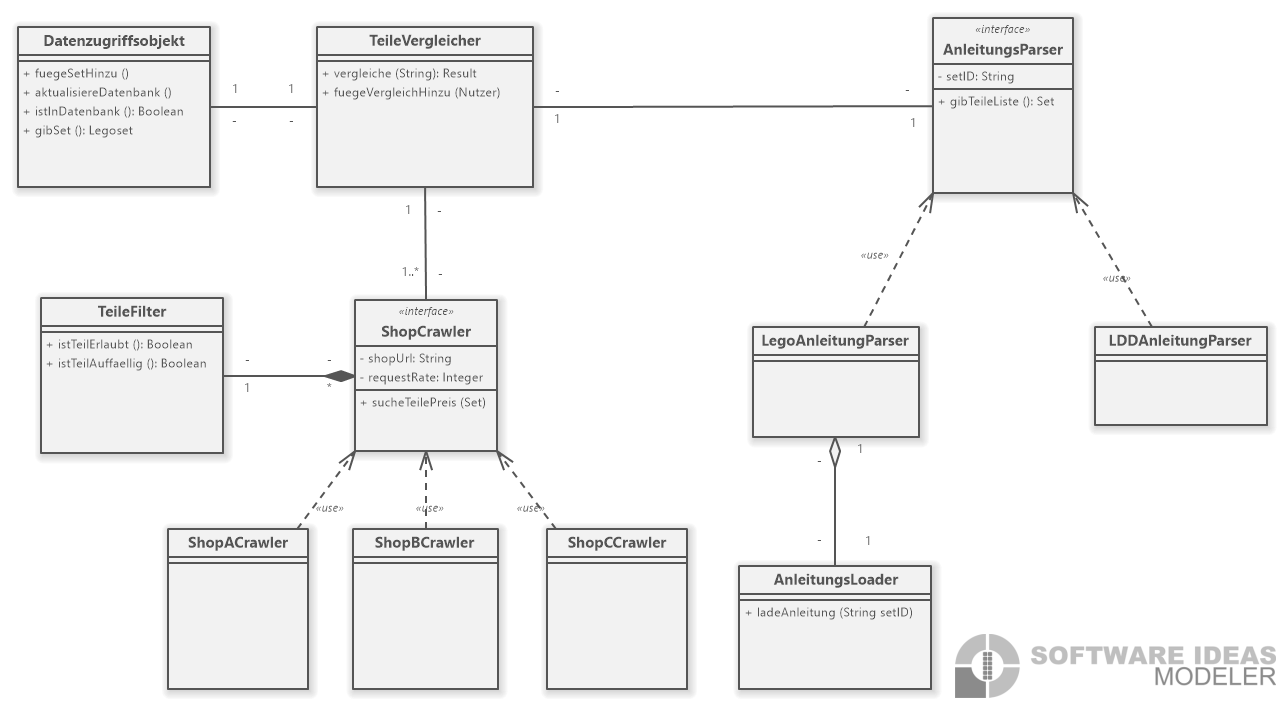
\includegraphics[width=18cm]{pictures/Architektur_Klassendiagramm.png}

\subsection{Benutzeraccount}
Benutzername \newline
Passwort (verschlüsselt) \newline
List: Suchhistorie \newline

\section{Produktleistungen}
Bestandsdatenbank soll aufgebaut werden mit Informationen aus den Anleitunge \newline
Preise sollen bei der Suche gecrawlt werden \newline
Die verwendete Datenbank muss in der Lage sein große Datenmengen zu speichern und zu verarbeiten \newline
Der Crawler soll in der Lage sein schnell Preisdaten bei den Anbietern zu crawlen, außerdem soll ein Algorithmus regelmäßig die neuen Anleitungen erkennen und dem Parser übergeben \newline

\section{Benutzungsoberfläche}

\includegraphics[width=18cm]{pictures/programmvorschau3.png}

\section{Technische Produktumgebung}
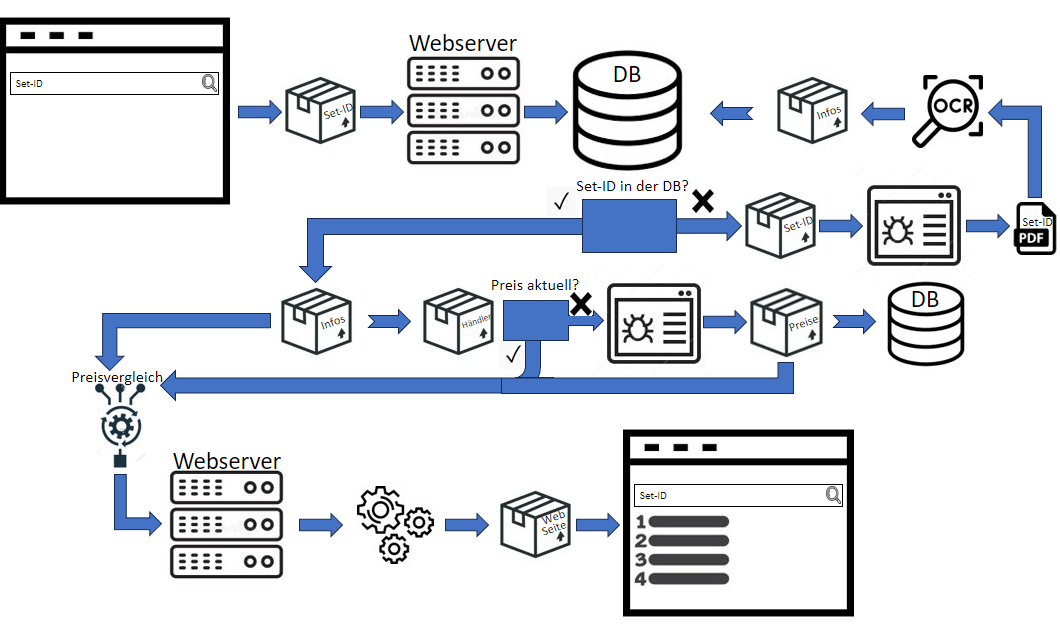
\includegraphics[width=18cm]{pictures/systemdurchlauf.png} \newline
Eine Datenbank wird mithilfe von SQLAlchemy in Python erstellt und aufgesetzt. Dies läuft auf einem Server mit xB Speicher, damit die ganzen Daten gespeichert werden können \newline
Es wird 1/2 Crawler erstellt in Python, die auf dem Server laufen. Diese dienen zur Suche von Preisen, so wie zur Suche der richtigen PDF \newline
Der Webserver ist jederzeit ansprechbar, damit Benutzer auf unser Tool jederzeit zugreifen können
OCR wird zum auslesen der PDF benutzt, damit die jeweilige Stückzahl und ID der Einzelteile herausgefunden werden kann \newline
Angular dient als Frameworkerstellungstool für eine interaktive Front End \newline
HTML und CSS zur Aufbesserung des Framework \newline
Python als primäre Programmiersprache, für alle Bereiche, wo programmiert werden soll \newline
Tex zur gemeinsame Dokumentation \newline
Git zum einfachen austausch von Fortschritt und jegliche andere Projekt relevante Erzeugnis \newline

\section{Gliederung in Teilprodukte}
\subsection{Crawler}
Die Klassen, welche das ShopCrawler Interface implementieren, besitzen die Logik einen Bestimmten Shop zu Crawlen. Für jeden berücksichtigten Shop wird eine Klasse benötigt, welche das Interface ShopCrawler implementiert.  Durch die Verwendung des Interfaces ist es möglich von unterschiedlichen Anbieter Webseiten die gecrawlten Ergebnisse in der gleichen Struktur zurückzugeben. Es ist möglich einen ShopCrawler ein Objekt der Klasse Filter zu übergeben, welcher es ermöglicht, beim Crawlen nach bestimmten Eigenschaften die Daten zu filtern.

\subsection{TeileFilter}
Der Teile Filter verfügt über Funktionen, welche auf die gecrawlten Daten angewendet werden und prüft, ob die Daten auf die Filtereigenschaften zutreffen.

\subsection{Anleitungsparser}
Das Interface Anleitungsparser liefert eine Struktur eines Parsers für Bauanleitungen. Dadurch ist gewährleistet, dass die Klassen, die das Interface implementieren die Geparste Anleitung in der Richtigen Struktur zurückgeben. Die Jeweiligen Klassen der Parser müssen zusätzlich eine OCR-Bibliothek einbinden, welche das auslesen von PDF Dateien ermöglicht. \newline 
\newline 
\subsection{Anleitungsloader}
Für das Parsen einer Anleitung muss die Anleitung aus dem Internet heruntergeladen werden, dies Ermöglicht der Anleitungsloader. Mit einem Web-Crawler findet er die PDF-Datei zu einer Angegebenen SetID und lädt diese herunter und stellt sie einer Anleitungsparser Implementierung zur Verfügung. \newline 
\newline 
\subsection{Datenzugriffsobjekt}
Das Datenzugriffsobjekt ermöglicht den Zugriff auf die Datenbank. Es besitzt die die nötigen Funktionen die notwendigen Objekte auf der Datenbank zu persistieren oder auf der Datenbank persistente Daten abzurufen. \newline 
\newline 
\subsection{Teilevergleicher}
Teilevergleicher ist die Zentrale Klasse im System.  Die Klasse besitzt die Funktion eine Suche zu starten und sie bündelt alle anderen Objekte im System. Sie bestimmt den logischen Ablauf der Ausführung der Suche.\newline 

\section{Globale Testfälle}
/T010/\newline 
Set suchen: Der Nutzer gibt in der Suchleiste die Lego-Setnummer 75355 ein. \newline
\newline
/T020/ \newline Historie anzeigen: Der Nutzer klickt auf "Historie" um sich seine persönliche Such-Historie anzeigen zu lassen. \newline
\newline
/T030/ \newline Registrieren: Der Nutzer klickt auf "Registrieren" und registriert sich mit den Daten \newline           
- Name: Max Mustermann \newline
- E-Mail: mustermann@gmx.de \newline                               
- Passwort: passwort \newline
\newline
/T040/ \newline 
Anmelden:  Der Nutzer klickt auf "Anmelden" und meldet sich mit den in /T30/ benannten Daten an.\newline
\newline
/T050/ \newline 
Stückliste anzeigen: Der Nutzer lässt sich die Stückliste anzeigen ? \newline
\newline
/T060/ \newline
Kommt aufs Design der Nutzeroberfläche an ?  \newline
\newline
/T100/ \newline
PDF crawlen: Der Nutzer gibt die Set-Nummer 75192 in die Suchleiste ein, welche noch nicht in der Datenbank liegt. Der Web-Crawler sucht die jeweilige PDF Anleitung des Lego Sets. \newline
\newline
/T110/ \newline
PDF auslesen: Nach /T100/ wird das entsprechende PDF-Dokument mittels OCR ausgelesen. \newline
\newline
/T120/ \newline
Einzeilteile in Datenbank speichern: Nach /T110/  werden die Nummern der Einzelteile korrekt in die Datenbank gespeichert. \newline
\newline
/T130/ \newline
Preise crawlen: Nach /T120/ werden die Preise auf den Händlerseiten je nach Set und Einzelteilen abgefragt und gespeichert. \newline
\newline
/T140/ \newline
Preise vergleichen: Nach  /T130/ findet ein Preisvergleich zwischen den Sets und Einzelteilen ab. Dies erfolgt für alle erfassten Händler. \newline
\newline
/T150/ \newline
Darstellung des Ergebnis-Fensters: Nach der Funktion /F100/ wird das nächste Fenster mit den entsprechenden Ergebnissen nach /F110/ - /F140/ angezeigt. \newline
\newline
/T160/ \newline
Benutzer verwalten: Der Admin löscht den Nutzer Max Mustermann aus /T030/. \newline
\newline
/T170/ \newline
Statistiken anzeigen: Der Admin Maxine Mustermann klickt auf die Einstellung "Dashboard" um sich Statistiken zu den Suchanfragen anzeigen zu lassen. \newline
\end{document}